\section{Mindfulness meditation}
%Definition
Mindfulness is often defined as being in the mental state of Non-Elaborative, non-judgmental awareness \cite{Zeidan2012,Zeidan2016}. 
Two popular practices of mindfulness meditation, focused attention (FA) and open monitoring (OM) are of the most well practiced types of meditation. 
Practicing mindfull meditation includes control over sensory, emotional and cognitive happenings. Hereby the ability control these sensations without being distracted by them and also abstract from past and future representations of memory.
%Effect

Very little mindfulness training can have an effect.. study by... showed an effect examined for 20 min sessions for 4 days of mindfulness meditation. 

FA and OM can alter pain in different ways...
OM is more effective in reducing pain after extensive meditation training compared to FA. 
\cite{Varilly2012}
%2 practices of mindfulness

\textbf{Focused attention}\\ 
FA is the training for concentration, where one keeps the focus to an object or specific thing, only focusing on that thing. Often the flow of breath is the focus, when practicing FA meditation.  When any disturbance comes by, like a thought, sound or other environmental distractions, which will often lead to a drift in attention, the person should always bring his or her attention back to the focus. 

This kind of meditation has shown to enhance focus and concentration. ..

\textbf{Open monitoring}\\
OM is the cultivation of open presence, were the mind is open to anything, not focusing on any specific thing, just being in the present. If any thought or disturbance comes by the thought or sensation should be let go without thinking more over it. It is believed that this form of meditation is easier to learn when one master the meditation of FA, whereby the OM meditation form is easier to master. 

This kind of meditation has been shown to reduce pain more compared to FA, likely because the areas of the brain affected during this form of meditation is...

\cite{Perlman2010}

\begin{figure}[H]
	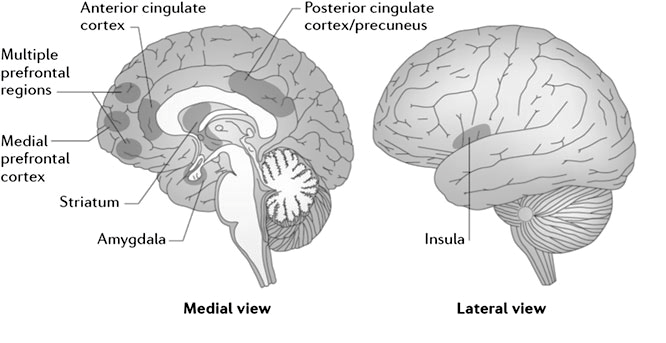
\includegraphics[width=.8\textwidth]{figures/brain_meditation} 
	\caption{Image of the brain and activation of specific brain regions when practicing meditation}
	\label{fig:brain_meditation}  
\end{figure}                                         


